\chapter{Uncertainties in the cross-section measurement}\label{chap:Unc}
\minitoc
Cross-section measurement relies on theoretical models and corrections, used in Monte-Carlo. Thus, their intrinsic uncertainties should be propagated to a final result. This chapter discusses main methods of uncertainties measurements and sources on $C_{W,Z}$ and $A_{W,Z}$ correction factors. 

\section{Methods of uncertainties propagation}
All sources of systematic uncertainties are propagated in these analyses using one of the main methods: Offset, On/Off or Toy Monte-Carlo. The offset method changes a correction by a $\pm 1\sigma$ of it's systematic uncertainty. The contribution of each correction's uncertainty on the observable (e.g. $C_{W,Z}$, $A_{W,Z}$ or a cross-section) is taken as a symmetric approximation:
\begin{equation}
U_i^{offset}=\frac{\sigma_{i}^{up}-\sigma_{i}^{down}}{2},
\end{equation}
where $\sigma_{i}^{up(down)}$ - the change in a observable due to the shift of the correction on $\sigma$ up or down. 

For On/Off method the contribution of each correction is estimated with ($\sigma^{on}$) and without($\sigma^{off}$) correction applied. A systematic error can be estimated than as:
\begin{equation}
U^{on/off}=\sigma^{on}-\sigma^{off}.
\end{equation}

Another one method used for a uncertainties propagation is a toy MC method, that uses a pseudo experiments with modified input corrections. For a scale factors binned $p_T$ and $\eta$ uncertainties inside each bin can be divided to a correlated  and uncorrelated systematic components and statistical error. For each pseudo-experiment, a table of new scale factors is filled, where inside each bin a scale factor is randomly varied as:
\begin{equation}\label{eq:ToyMethod}
SF_{i}^{Toy_{n}} = SF_{i}+ Gauss(0,\Delta SF_{i} ^{uncorr+stat}) + \sum \Delta SF_{i} ^{corr} \cdot Gauss(0, 1),
\end{equation}
where $SF_{i}^{Toy_{n}}$ is a new scale factor in i-th bin, $\Delta SF_{i} ^{uncorr+stat}$ - is the quadratic sum of uncorrelated and statistical errors and $\Delta SF_{i} ^{corr}$ is a correlated error.

The overall effect on a observable is calculated as a standard deviation of the values in a pseudo-experiments:
\begin{equation}\label{eq:ToyError}
U_{i}=\sqrt{\frac{\sum_{Toy_n=1}^{N} \sigma^2_{i}} {N} - \Bigg(\frac{\sum_{Toy_n=1}^{N} \sigma_{i}} {N}\Bigg)^2}
\end{equation}
The number N of pseudo experiments should be sufficiently large to avoid possible bias in the uncertainty estimation.
 
\section{Experimental systematic uncertainties}
Sources of experimental uncertainties, methods of estimation and their effect on a $C_{W,Z}$ are summarized in a Tab. \ref{tab:Unc}. Systematical errors coming from a hadron recoil calculation are discussed in a Sec. \ref{sec:HadrCalib}. 
\subsection{Electron energy scale and resolution}
Electron energy scale correction, described in Sec. \ref{sec:elecScale} has associated uncertainties coming from \cite{1110.3174}:
\begin{itemize}
\item Statistical component of the scale uncertainty
\item Uncertainty from the possible bias of the calibration method
\item Scale uncertainty from the choice of generator
\item Uncertainty from the presampler energy scale
\item Imperfect knowledge of the material in front of EM calorimeter.
\end{itemize}
The uncertainty contribution from each component is estimated using offset method. The total energy scale uncertainty is the quadratic sum of the components \cite{ElecUncQuad}. 

\subsection{Muon energy scale and resolution}
Systematic uncertainties coming from muon momentum corrections described in Sec. \ref{sec:MuonMomCor} can be divided into 3 major independent categories:
\begin{itemize}
\item variations of the smearing of MS track
\item variation of the smearing of ID track
\item overall scale uncertainty
\end{itemize}
The uncertainty contribution from each component is estimated using offset method. The total energy scale uncertainty is the quadratic sum of the components.

\subsection{Muon and electron efficiency toy Monte-Carlo}
 In case of 2.76 TeV analysis scale factor errors are considered to be enlarged for a statistical and uncorrelated components, so correlated error is assumed to be negligible. The toy MC experiments are performed for electron reconstruction, identification and trigger scale factors and muon reconstruction + identification scale factors.  In the current analysis 30 pseudo-experiments are used with a combined toy MC method. 
 
 \subsection{Theoretical uncertainty}\label{sec:TheoCw}
 
 The theoretical uncertainty considered to be coming from imperfect knowledge of parton functions and is calculated as:
 \begin{itemize}
 \item  Error coming from an arbitrary choice of PDF set is estimated by PDF reweighting \cite{PDFRew} of original MC generated using CT10 PDF set to a one of the 4 pdf sets: ATLAS-epWZ12 \cite{ATLASEP}, abkm09\cite{ABM09} and NNPDF23\cite{NNPDF23}. The error is calculated as a maximum deviation between the acceptance calculated CT10 and different PDF set. 
\item Systematic uncertainty within one pdf set  is evaluated using CT10 NLO set. This set contains 52 asosiated error sets, corresponding to a 90\% C.L. limits along 26 eigenvectors. The resulting 52 variation are separetelly added in a quadrature as:
\begin{equation}\label{eq:PDF}
\delta_X=\frac{1}{2}\cdot \sqrt{\sum_{i=1}^{N}(X^+-X^-)^2}
\end{equation}
\end{itemize}
 
 \newcommand{\rot}{\rotatebox{90}}
\newcommand\tab[1][1cm]{\hspace*{#1}}

\begin{landscape}
\begin{table}[p]
\caption{}
\label{tab:Unc}
\begin{center}
\begin{tabular}{l | c  || c | c || c | c || c | c ||  }
Source of uncertainty & Method & $\delta C_{W} / C_{W} (\%) $ & $\delta C_{W} / C_{W} (\%) $ & $\delta C_{W} / C_{W} (\%) $ & $\delta C_{W} / C_{W} (\%) $ & $\delta C_{Z} / C_{Z} (\%) $ & $\delta C_{Z} / C_{Z} (\%) $\\
 &  & $W^{+}\to e\nu$ & $W^{-}\to e\nu$ & $W^{+}\to \mu\nu$ & $W^{+}\to \mu\nu$ & $Z\to ee$ & $Z\to \mu\mu$ \\
\hline
Electron reconstruction & Toy MC &  \RecEffToyWplusenu  & \RecEffToyWminenu & - & - & \RecEffToyZee  & - \\
Electron identification  & Toy MC &  \IDEffToyWplusenu  & \IDEffToyWminenu &  - & -  & \IDEffToyZee  &  - \\
Electron trigger efficiency & Toy MC &  \TrigToyWplusenu  & \TrigToyWminenu & - & -  & \TrigToyZee  & - \\ 
Muon reco+id & Toy MC &  -  & - & \muIDEffToyWplusmunu & \muIDEffToyWminmunu   & - & \muIDEffToyZmumu \\
Muon trigger  & Offset&  -  & - & \muTrigWplusmunu & \muTrigWminmunu & - & \muTrigZmumu \\
Electron energy scale & Offset &  &  & - & - &  & -\\
\tab - Statistical error & Offset &  &  & - & - &  & -\\
\tab - Bias in method  & Offset &  &  & - & - &  & -\\
\tab - Scale uncertainty &  Offset&  &  & -  & - &  & -\\
\tab - Presampler energy scale & Offset &  &  &-  & - &  &- \\
\tab - Material knowledge &  Offset &  &  & - & - &  &- \\
Electron energy resolution & Offset &\SmearWplusenu  & \SmearWminenu & - & - & \SmearZee  &- \\
Muon energy scale & Offset & - & - & \MuSmearingScaleWplusmunu & \MuSmearingScaleWplusmunu & - & \MuSmearingScaleZmumu \\
Muon energy resolution total & Offset &- & - & Wplusmunu & Wminmunu & - & Zmumu\\ 
\tab - Muon ID energy scale & Offset & - & - & \MuSmearingMSWplusmunu & \MuSmearingMSWminmunu & - & \MuSmearingMSZmumu\\ 
\tab - Muon MS energy scale & Offset & - & - & \MuSmearingIDWplusmunu & \MuSmearingIDWminmunu & - & \MuSmearingIDZmumu\\ 
Hadron recoil scale & Offset &  &  &  &   & - & -\\
Hadron recoil resolution & Offset &  &  &  &  & - & - \\
EWK + $t\bar{t}$ background &  &  &  &  &  &  & \\
QCD  &  &  &  &  & - & - & \\
\hline
PDF error & &  &  &  &  &  & \\
\hline
Total& &  &  &  &  &  & \\
\hline
Statistics & &  &  &  &  &  & \\
\hline
Luminosity & &  &  &  &  &  & \\
\end{tabular}
\end{center}
\end{table}
\end{landscape}


\section{Theoretical uncertainty on $A_{W/Z}$ and $E_{W/Z}$ factors}
\begin{table}[!t]
\caption{Acceptance values (A) and extrapolation values (E) and their relative uncertainties in percent for W and Z production in electron and muon channels. The various components of the uncertainties are defined in the text. The total uncertainties ($\delta A_{tot}$ and $\delta E_{tot}$ ) are obtained as the quadratic sum of the three parts.}
\label{tab:AErr}
\begin{center}
\begin{tabular}{l | c  | c | c | c | c  }
\hline
\hline
& $A$ & $\delta A^{pdf}_{err}$  & $\delta A^{pdf}_{sets}$  & $\delta A_{hs+ps}$  & $\delta A_{tot}$  \\
\hline
$W^{+}$ & &\WplusenuAEigUp & \WplusenuAPDFUp & 0.9 & 0.9 \\
$W^{-}$ & & \WminenuAEigUp & \WminenuAPDFUp &  0.9 &  0.9\\
$Z$ & &\ZeeAEigUp & \ZeeAPDFUp & 0.9 &  0.9 \\
\hline
& $E$ & $\delta E^{pdf}_{err}$  & $\delta E^{pdf}_{sets}$  & $\delta E_{hs+ps}$  & $\delta E_{tot}$  \\
\hline
$W^{+}$ &  & \WminenuEEigUp &\WminenuEPDFUp & 0.7 & 0.7\\
$W^{-}$ & & \WminenuEEigUp &\WminenuEPDFUp & 1.0 & 1.0 \\
$Z$ & & \ZeeEEigUp & \ZeeEPDFUp & 1.0 & 1.0 \\
\hline
\hline
\end{tabular}
\end{center}
\end{table}

The effect of theoretical uncertainties must be considered for extrapolated cross-sections, through it effect on extrapolation factors $A_{W,Z}$, $E_{W,Z}$  factors. They are estimated taking into accound different independent contributions:
\begin{itemize}
\item  Error coming from an arbitrary choice of PDF set and systematic error within one pdf set is estimated in the same way, as for $C_W$ (see Sec. \ref{sec:TheoCw}). These sources are considered to be independent and added in a quadrature. 

\item The uncertainties arising from the choise of generator and parton showering model $\delta A_{hs+ps}$ are considered small. They can be calculated as a difference in the acceptances  $A_{W,Z}$ for MC samples, generated using same PDF set, but different models for showering and matrix element, namely Powheg + Pythia and Sherpa. The systematic error obtained for W channels is 0.9\% for $A_{W}$. It is consistent with 13 TeV and 7 TeV measurements.

 Because of the lack of simulation samples for $Z\to ll$ using Sherpa generator a systematic uncertainty for Z is estimated using the fact, that for 13 TeV analysis and 8 TeV systematic errors coming from that source have been the same for $A$-factors in $W^{+}$, $W^-$ and $Z$.
\end{itemize}

The overall theoretical systematic uncertainty on A and E factors are summarised in Tab. \ref{tab:AErr} and  factor.


 
\section{Correlation between uncertainties}\label{sec:Cor}

In order to calculate W/Z ratios and combine channels different channels of the analysis it is crucial to take into account correlations between different channels. In this sections the assumptions about correlations between channels will be discussed.

The theoretical uncertainties on A and C factors, except for the uncertainty within 1 pdf set are considered to be fully correlated between all analysis. The uncertainties within 1 pdf set are considered to be partially correlated (see Sec. \ref{sec:partCor}). The systematic uncertainties from electroweak background sources are treated as uncorrelated between W and Z channels and 100\% correlated for different W and Z channels.  

In addition to electroweak background uncertainty the following systematic sources are considered to be fully correlated between $W^{+}\to e\nu$, $W^{-}\to e\nu$, $W^{+}\to \mu \nu$ and $W^{-}\to \mu \nu$:
\begin{itemize}
\item QCD background 
\item Hadronic recoil scale
\item Hadronic recoil resolution
\end{itemize}

In addition to the mentioned systematics, the following uncertainties are considered 100\% correlated in electron analyses:
\begin{itemize}
\item Electron energy scale
\item Electron resolution
\end{itemize}
and in muon analyses:
\begin{itemize}
\item Muon energy scale
\item Muon resolution
\item Muon trigger efficiency
\end{itemize}

The uncertainties, estimated using toy MC method are considered partially correlated and a covariances between the analyses are estimated in the following section.

\begin{figure}[!p]
\begin{minipage}[h]{0.49\linewidth}
\center{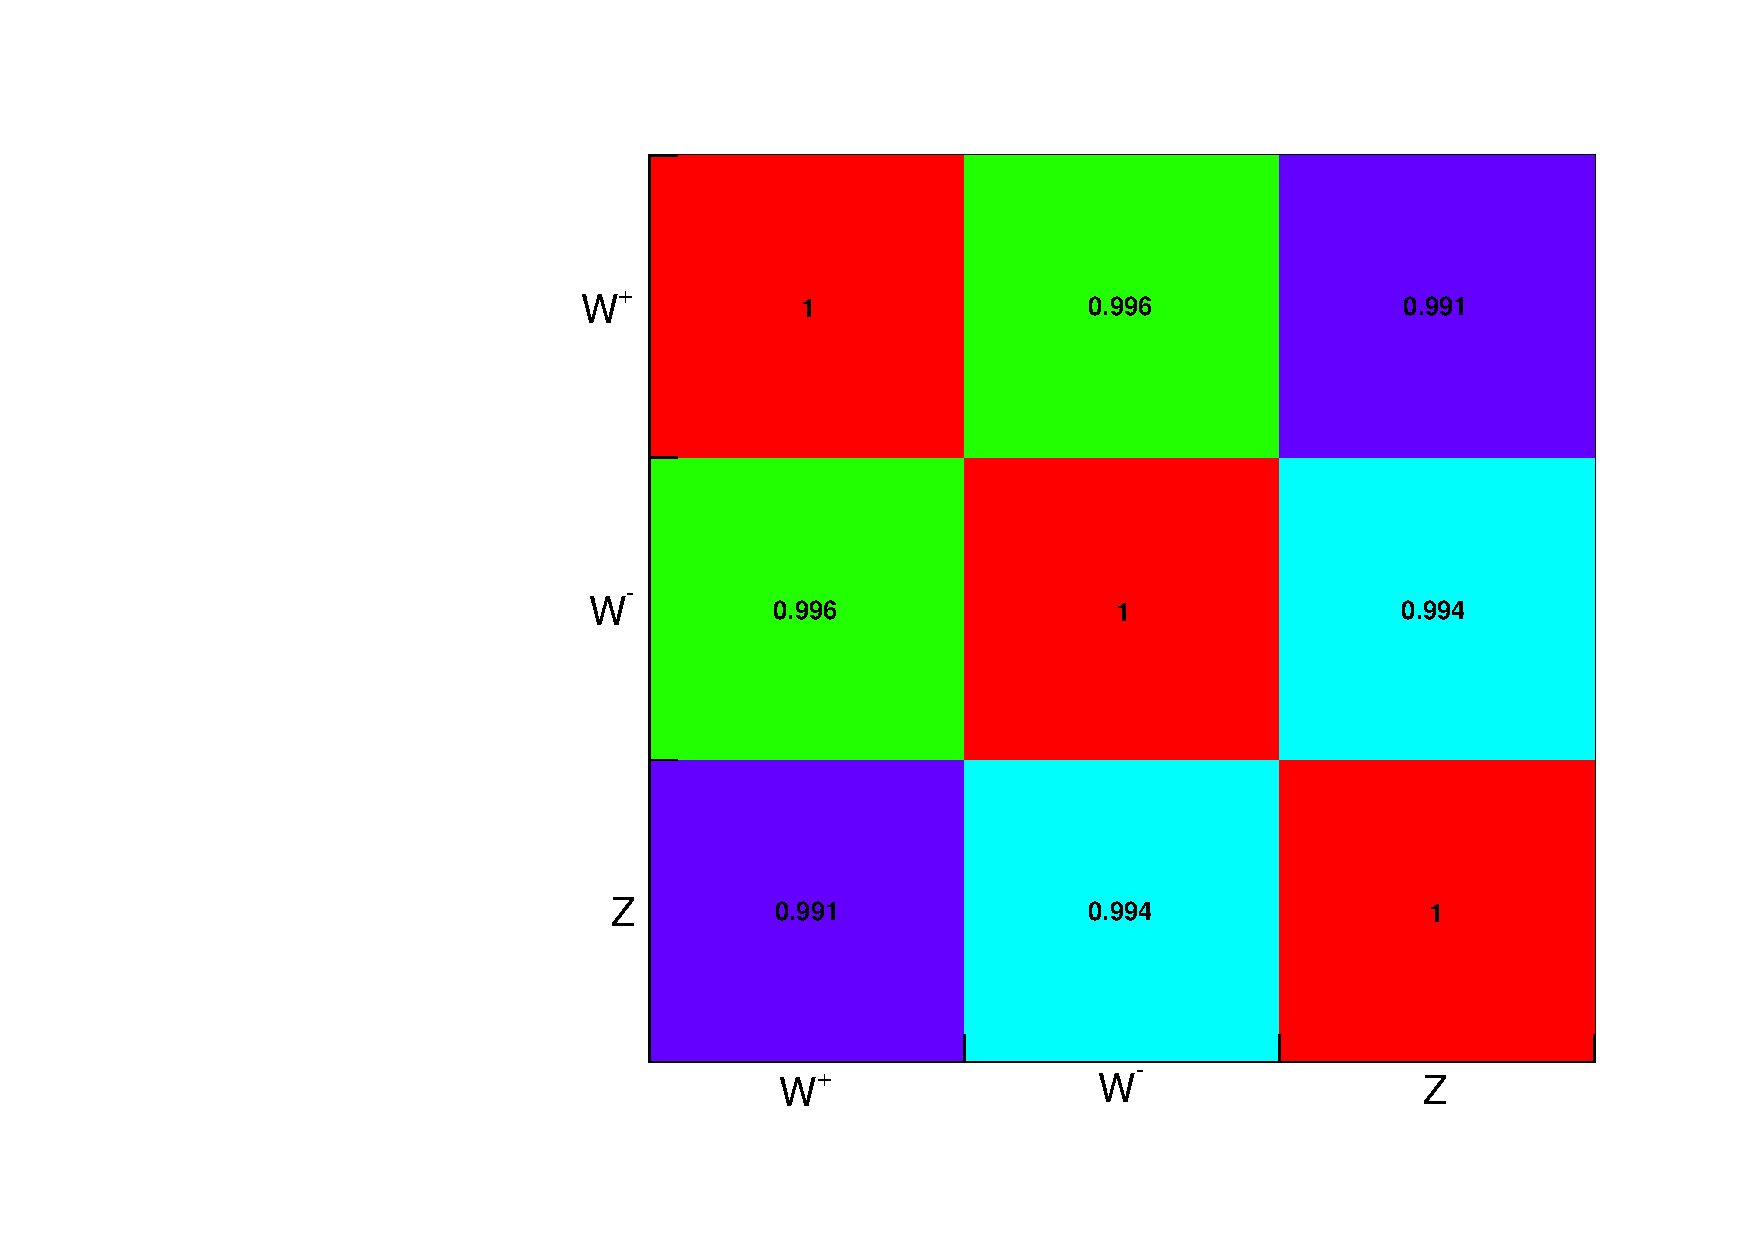
\includegraphics[width=1.0\linewidth]{Systematics/rec.pdf}  \\ a)}
\end{minipage}
\hfill
\begin{minipage}[h]{0.49\linewidth}
\center{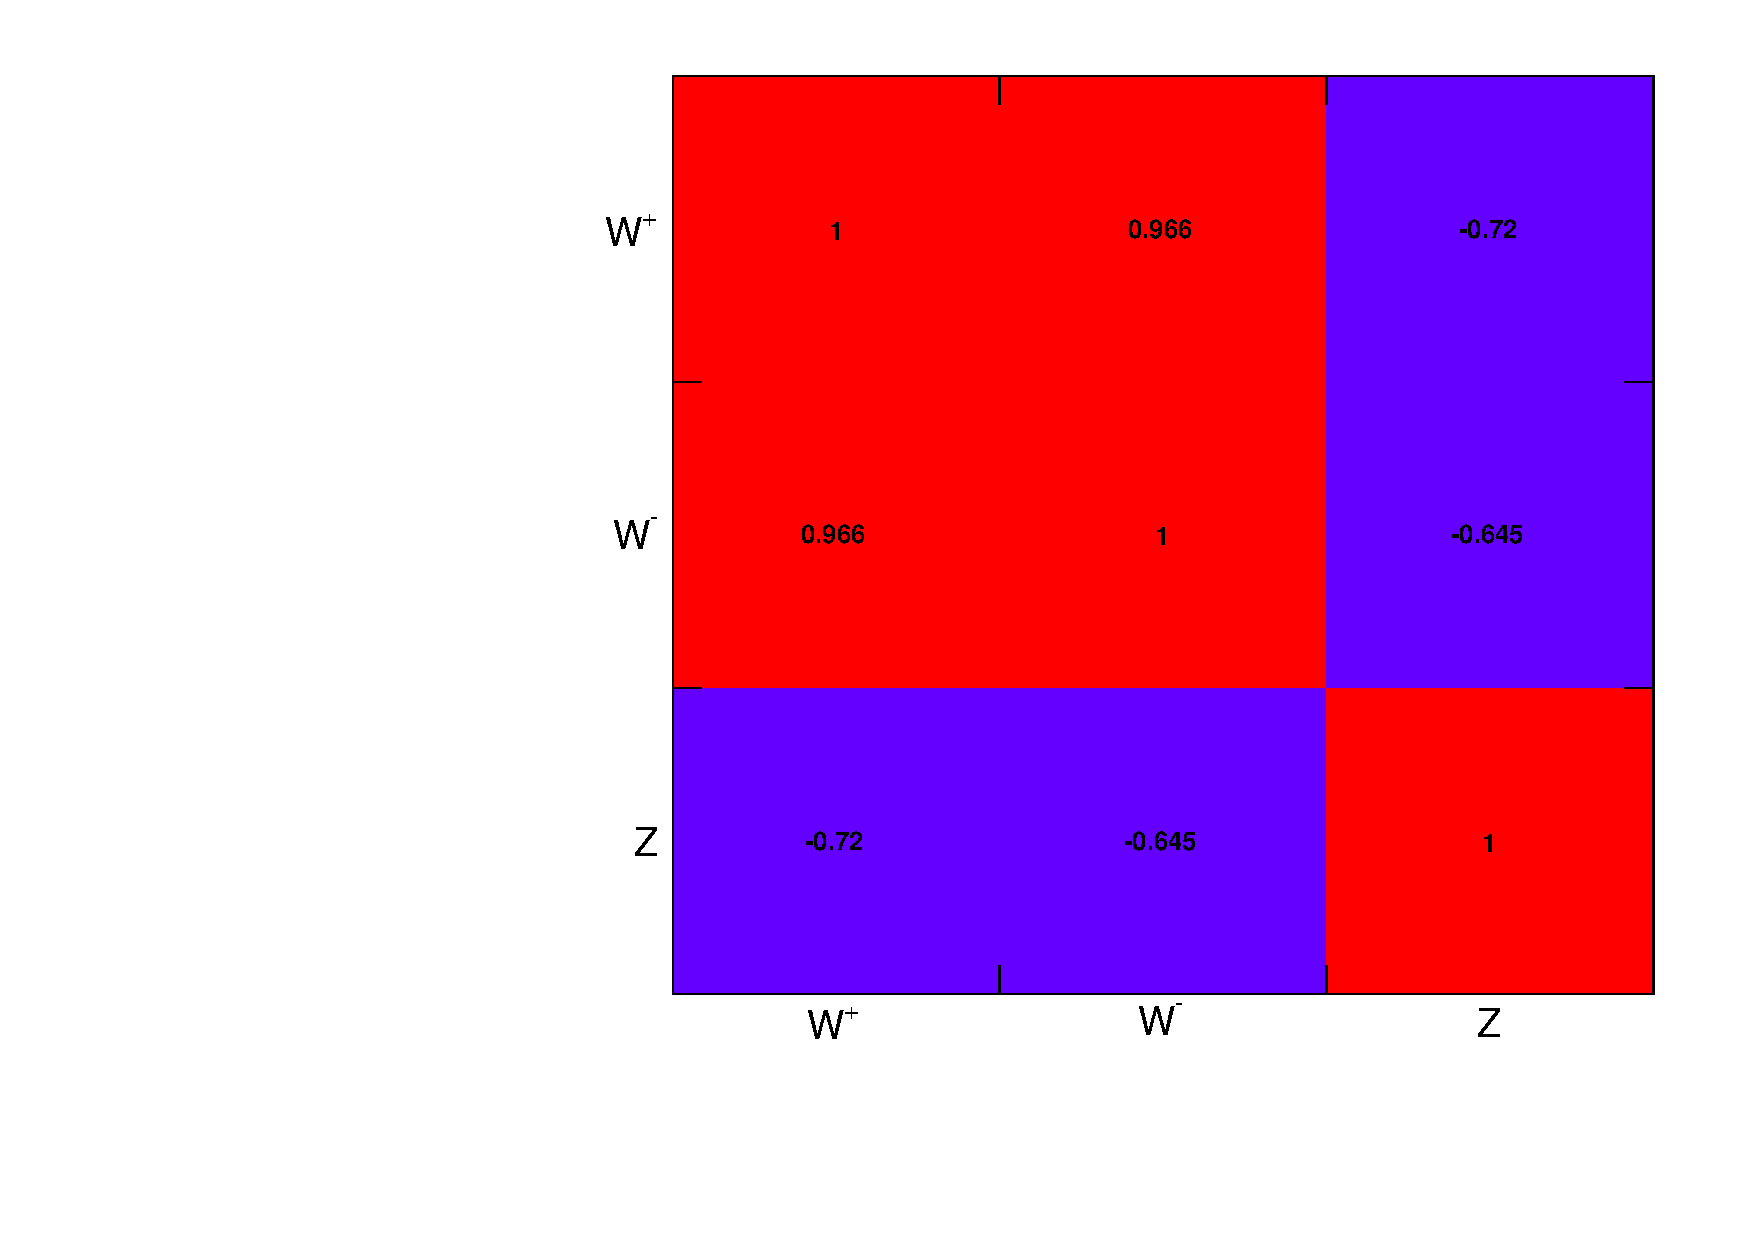
\includegraphics[width=1.0\linewidth]{Systematics/id.pdf} \\ b)}
\end{minipage}
\vfill
\begin{minipage}[h]{0.49\linewidth}
\center{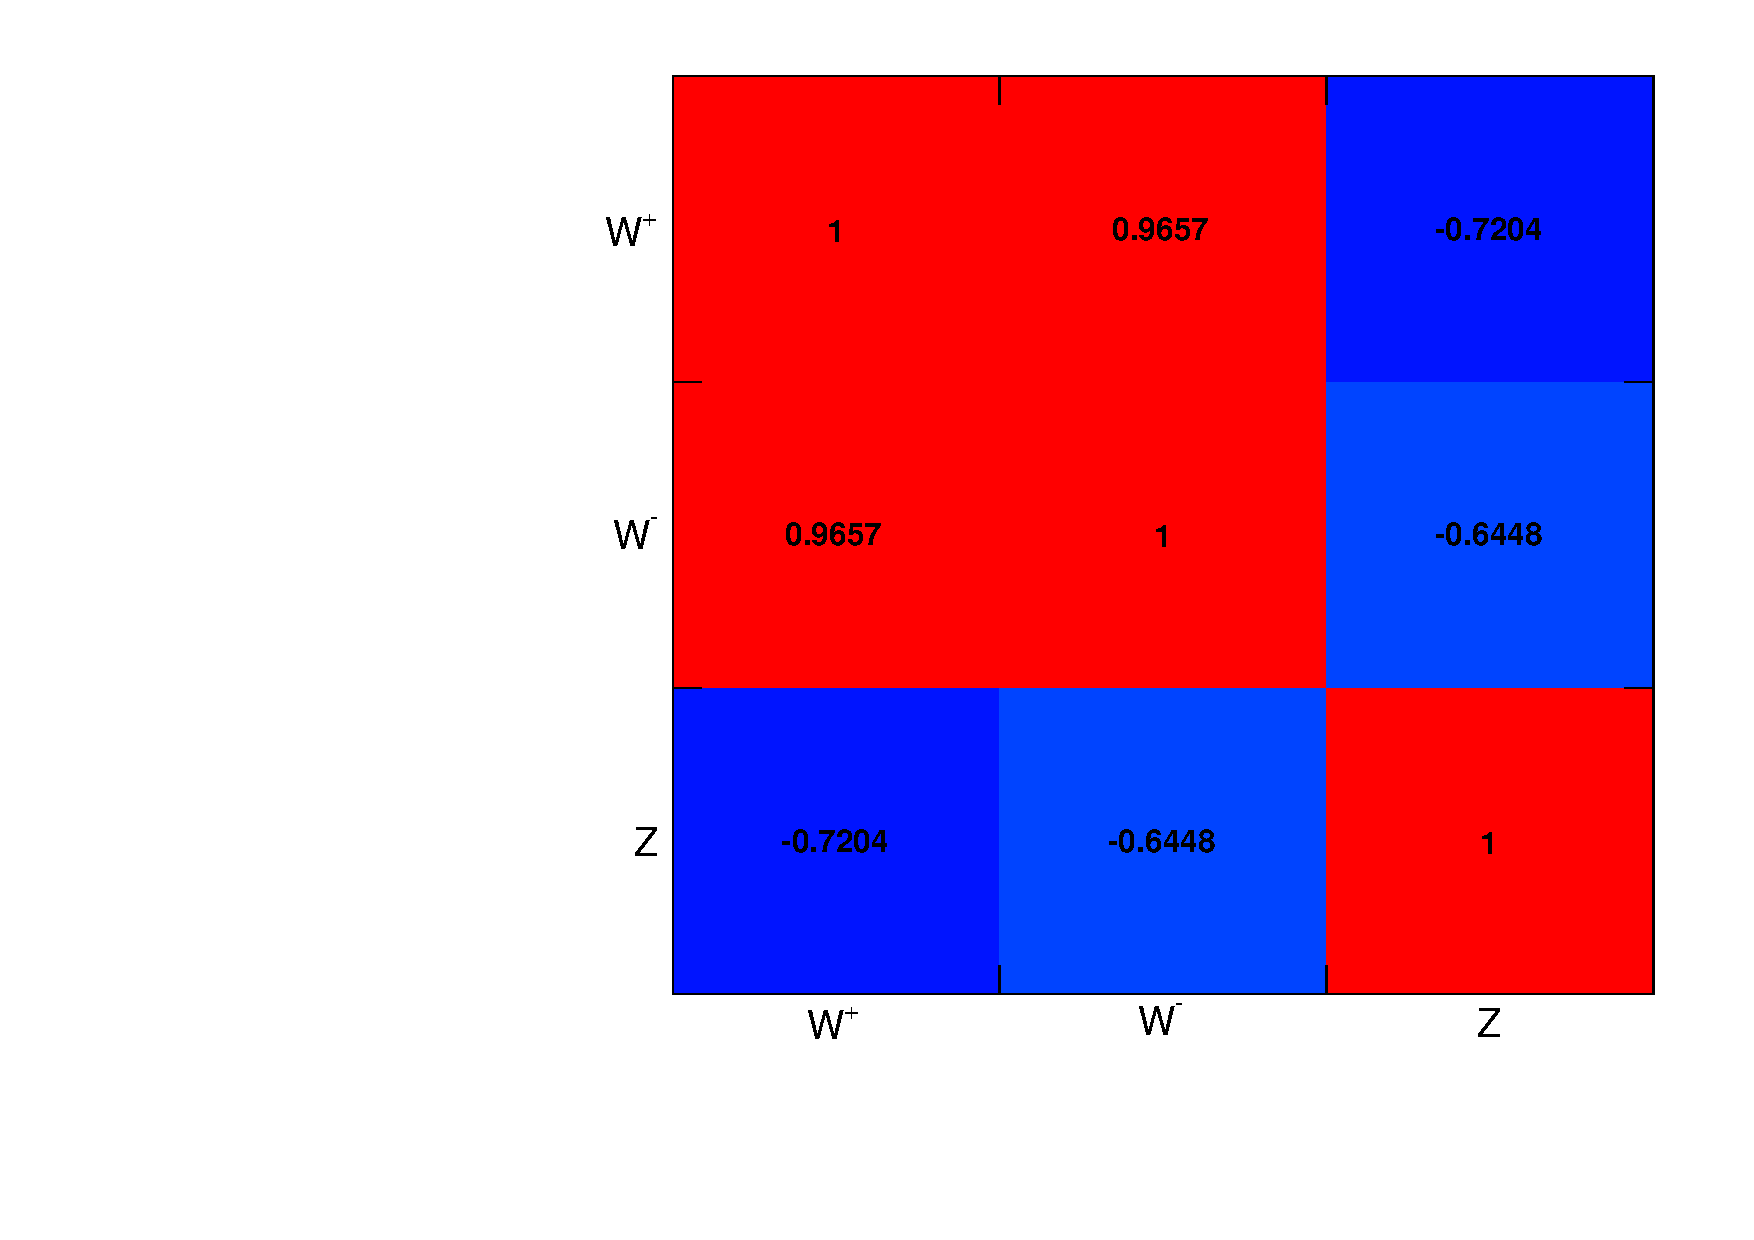
\includegraphics[width=1.0\linewidth]{Systematics/trig.pdf}  \\ c)}
\end{minipage}
\hfill
\begin{minipage}[h]{0.49\linewidth}
\center{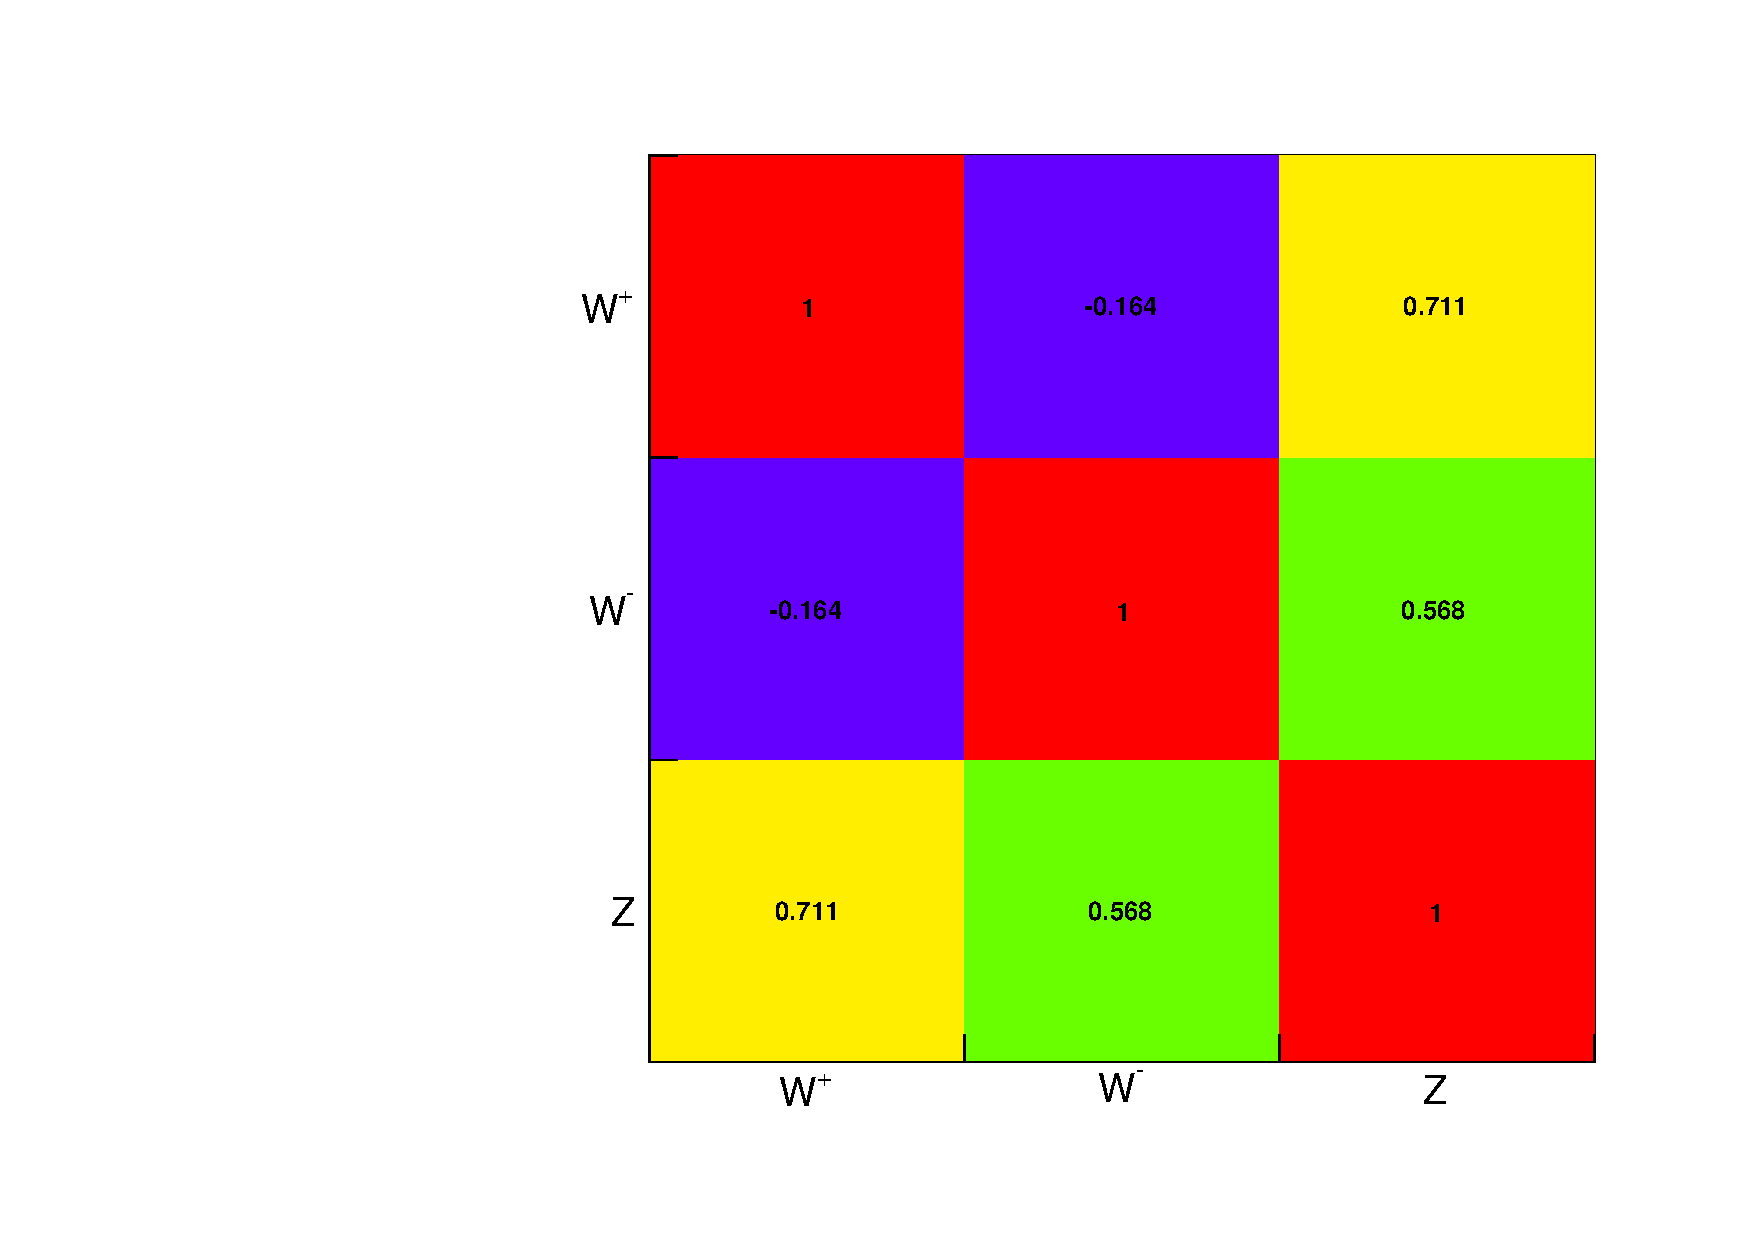
\includegraphics[width=1.0\linewidth]{Systematics/muID.pdf} \\ d)}
\end{minipage}
\caption{Correlation coefficients among $C_{Z}$ , $C_{W^{+}}$ and $C_{W^{-}}$   for a) electron reconstruction, b) electron identification, c) electron trigger and d) muon trigger scale factor uncertainties.}
\label{fig:CorToy}
\end{figure}

\subsection{Treatment of partially correlated uncertainties}\label{sec:partCor}

The following uncertainties are considered to be partially correlated between $Z$, $W^{+}$ and $W^{-}$ analyses for an observables $o_X$ and $o_Y$:
\begin{itemize}
\item Electron trigger efficiency
\item Electron resolution efficiency
\item Electron identification efficiency
\item Muon reconstruction + identification efficiency
\item Uncertainties within 1 pdf set
\end{itemize}

For each source of uncertainty a correlation coefficients between analysis X and Y can be estimated as:
\begin{equation}\label{eq:Corr}
\rho_{XY}=\frac{1}{\sigma(o_X)\sigma(o_Y)}\cdot \frac{1}{N} \sum_{i=1}^N (o^i_X-\bar{o}_X) (o^i_Y-\bar{o}_Y)=\frac{C_{XY}}{\sigma(o_X)\sigma(o_Y)},
\end{equation}
where $\bar{o}_X$ and $\bar{o}_Y$ are the mean values of $o_X$ and $o_Y$ respectivelly,  $\sigma(o_X)$ and $\sigma(o_Y)$ are the uncertainties and $i$ is the number of experiment.  The $C_{XY}$ denotes elements of the covariance matrix. Resulting correlation matrices for each toy MC systematic source are shown in Fig.~\ref{fig:CorToy}.



Correlation coefficients for a systematic error within 1 pdf set are considered independent for each eigenvectors. Using the Eq.~\ref{eq:Corr} and \ref{eq:PDF} the total correlation matrix $C^{PDF}_{XY}$ can be calculated as:
\begin{equation}
C^{PDF}_{XY}= \frac{1}{4}\sum(X^{+}-X^{-})\cdot (Y^{+}-Y^{-}).
\end{equation}
The resulting covariance matrix for an A factor is shown in Fig. \ref{fig:ApdfErr}.

\begin{figure}[!tb]
\begin{center}
\begin{minipage}[h]{0.49\linewidth}
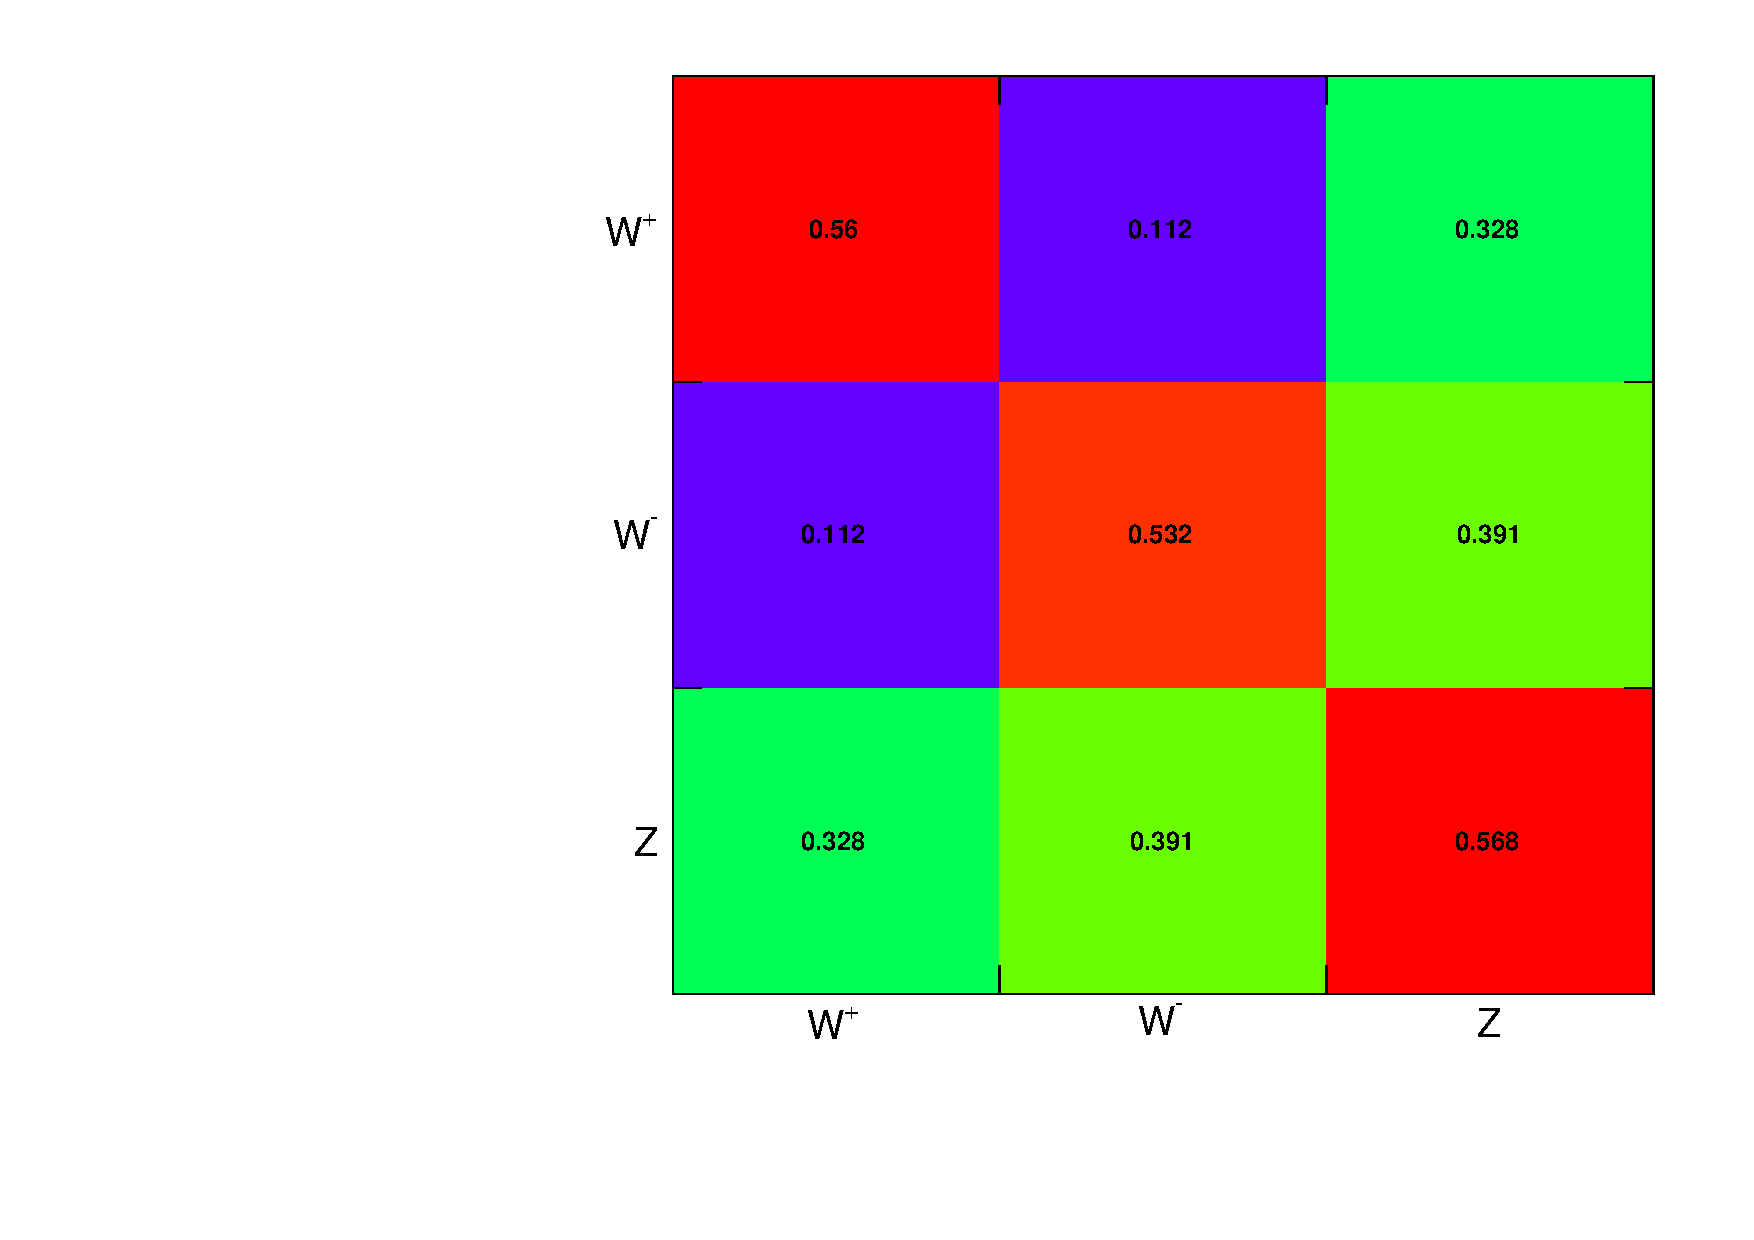
\includegraphics[width=1\textwidth]{Systematics/ePDF.pdf}
\end{minipage}
\caption{Covariance coefficients among $A_{Z}$ , $A_{W^{+}}$ and $A_{W^{-}}$ for the PDF uncertainty within 1 pdf set}
\label{fig:ApdfErr}
\end{center}
\end{figure}

The covarinace matrix C, using Cholesky decomposition\cite{Dickinson1978} can be re-written as:
\begin{equation}
C=L \cdot L^{T},
\end{equation}
where $L$ is a lower triangular matrix, and $L^{T}$ is a transpose of L. Because the covariance matrix has a positive definitive this matrix is always unique. 
Rows of the matrix L are corresponding to an systematic error vectors, that are fully correlated between $W^{+}$, $W^{-}$ and $Z$ analyses. This allows the coherent treatment of the correlated uncertainties.



